\begin{table*}[!t]
    \centering
    \footnotesize
    \begin{minipage}[t]{0.56\textwidth}
        \centering
    \caption{Analysis experiment results on ScreenSpot-pro. \textbf{Relax@k} measures how many previously incorrect offset predictions are recovered when the ground-truth bounding box is expanded by k visual patches along each dimension. \textbf{Corrected} refers to the number of offset predictions corrected by the second step, while \textbf{Lost} refers to the number of predictions that degrade after the second step.}
    % \vspace{-0.5em}
    \resizebox{\linewidth}{!}{
    % \begin{tabular}{y{160}cccccc}
    \begin{tabular}{lcccc|cc|c}
        \toprule
        Model& Relax@1 & Relax@3 & Relax@5 & \textbf{Total} & \textbf{Corrected} & \textbf{Lost}&\textbf{Improved} \\
        \midrule
        \rowcolor{gray!30}
        \multicolumn{8}{l}{\textit{1-step}} \\
        Origin 1-step & 158 & 92 & 56 & 306 & - & - &-\\
        \midrule
        \rowcolor{gray!30}
        \multicolumn{8}{l}{\textit{2-step}} \\
        Crop-only & 123 & 83 & 43 & 249 & 156 & 107 &49\\
        Crop + 1.5$\times$Zoom-in & 47 & 74 & 38 & 159 & 208 & 48 & 160\\
        Crop + 2$\times$Zoom-in& 39 & 63 & 45 & 147 & 215&33& \bf 182  \\
        Crop + 3$\times$Zoom-in& 39 & 69 & 44 & 152 &219 & 42&177 \\
        Crop + 4$\times$Zoom-in& 31 & 72 & 38 & 141 &224 & 48&176\\
        \bottomrule
      \end{tabular}}
    % \vspace{-2.5em}
    \label{tab:analysis_zoom}
\end{minipage}
    \hfill
    \begin{minipage}[t]{0.4\textwidth}
    \captionsetup{type=figure}
    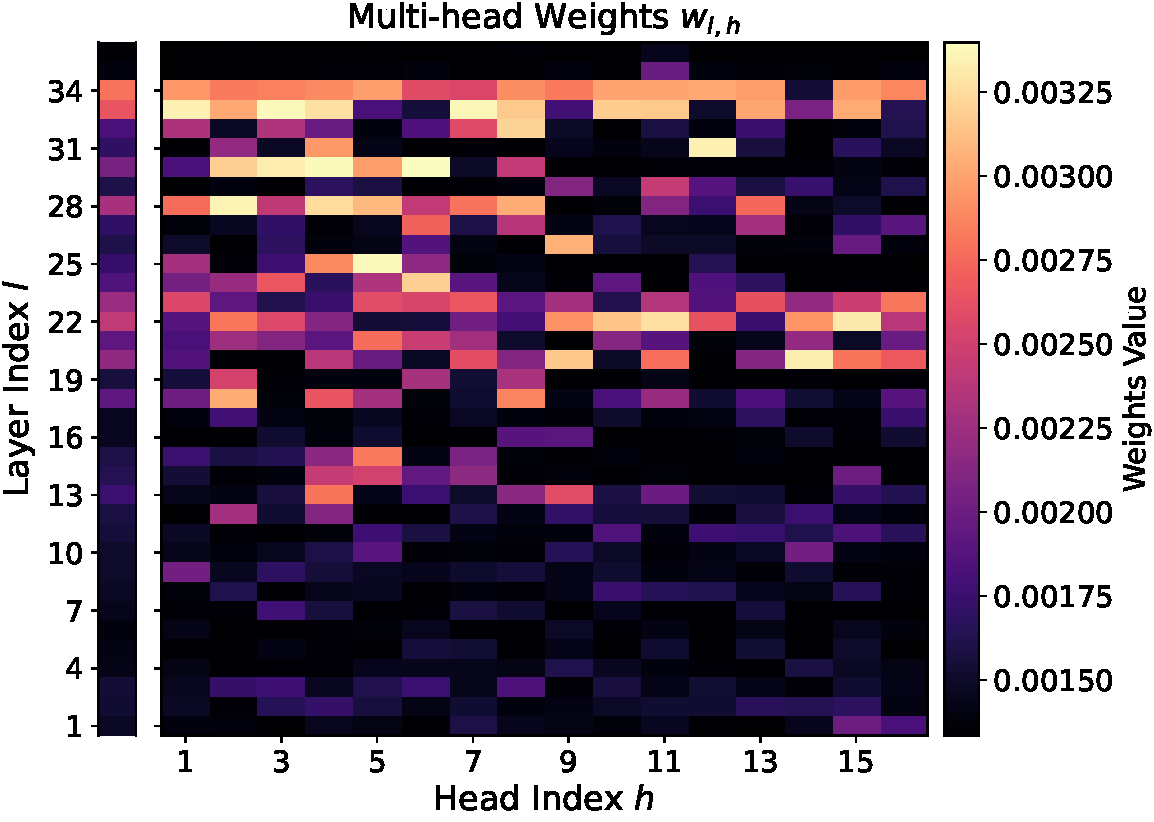
\includegraphics[width=0.9\linewidth]{fig/ALL_mean_headweights.pdf}
    \vspace{-1em}
    \caption{Visualization of multi-head weights $w_{l,h}$ averaged over the ScreenSpot-Pro, ScreenSpot-v2 and OS-World-G. \textbf{Left:} layer-wise mean, i.e., for layer $l$: $\frac{1}{H}\sum_{h=1}^{H}w_{l,h}$. \textbf{Right:} per-layer, per-head weights $w_{l,h}$.
    }
    \label{fig:contribution_head}
    \end{minipage}
\end{table*}